% Options for packages loaded elsewhere
% Options for packages loaded elsewhere
\PassOptionsToPackage{unicode}{hyperref}
\PassOptionsToPackage{hyphens}{url}
\PassOptionsToPackage{dvipsnames,svgnames,x11names}{xcolor}
%
\documentclass[
  letterpaper,
  DIV=11,
  numbers=noendperiod]{scrreprt}
\usepackage{xcolor}
\usepackage{amsmath,amssymb}
\setcounter{secnumdepth}{5}
\usepackage{iftex}
\ifPDFTeX
  \usepackage[T1]{fontenc}
  \usepackage[utf8]{inputenc}
  \usepackage{textcomp} % provide euro and other symbols
\else % if luatex or xetex
  \usepackage{unicode-math} % this also loads fontspec
  \defaultfontfeatures{Scale=MatchLowercase}
  \defaultfontfeatures[\rmfamily]{Ligatures=TeX,Scale=1}
\fi
\usepackage{lmodern}
\ifPDFTeX\else
  % xetex/luatex font selection
\fi
% Use upquote if available, for straight quotes in verbatim environments
\IfFileExists{upquote.sty}{\usepackage{upquote}}{}
\IfFileExists{microtype.sty}{% use microtype if available
  \usepackage[]{microtype}
  \UseMicrotypeSet[protrusion]{basicmath} % disable protrusion for tt fonts
}{}
\makeatletter
\@ifundefined{KOMAClassName}{% if non-KOMA class
  \IfFileExists{parskip.sty}{%
    \usepackage{parskip}
  }{% else
    \setlength{\parindent}{0pt}
    \setlength{\parskip}{6pt plus 2pt minus 1pt}}
}{% if KOMA class
  \KOMAoptions{parskip=half}}
\makeatother
% Make \paragraph and \subparagraph free-standing
\makeatletter
\ifx\paragraph\undefined\else
  \let\oldparagraph\paragraph
  \renewcommand{\paragraph}{
    \@ifstar
      \xxxParagraphStar
      \xxxParagraphNoStar
  }
  \newcommand{\xxxParagraphStar}[1]{\oldparagraph*{#1}\mbox{}}
  \newcommand{\xxxParagraphNoStar}[1]{\oldparagraph{#1}\mbox{}}
\fi
\ifx\subparagraph\undefined\else
  \let\oldsubparagraph\subparagraph
  \renewcommand{\subparagraph}{
    \@ifstar
      \xxxSubParagraphStar
      \xxxSubParagraphNoStar
  }
  \newcommand{\xxxSubParagraphStar}[1]{\oldsubparagraph*{#1}\mbox{}}
  \newcommand{\xxxSubParagraphNoStar}[1]{\oldsubparagraph{#1}\mbox{}}
\fi
\makeatother


\usepackage{longtable,booktabs,array}
\usepackage{calc} % for calculating minipage widths
% Correct order of tables after \paragraph or \subparagraph
\usepackage{etoolbox}
\makeatletter
\patchcmd\longtable{\par}{\if@noskipsec\mbox{}\fi\par}{}{}
\makeatother
% Allow footnotes in longtable head/foot
\IfFileExists{footnotehyper.sty}{\usepackage{footnotehyper}}{\usepackage{footnote}}
\makesavenoteenv{longtable}
\usepackage{graphicx}
\makeatletter
\newsavebox\pandoc@box
\newcommand*\pandocbounded[1]{% scales image to fit in text height/width
  \sbox\pandoc@box{#1}%
  \Gscale@div\@tempa{\textheight}{\dimexpr\ht\pandoc@box+\dp\pandoc@box\relax}%
  \Gscale@div\@tempb{\linewidth}{\wd\pandoc@box}%
  \ifdim\@tempb\p@<\@tempa\p@\let\@tempa\@tempb\fi% select the smaller of both
  \ifdim\@tempa\p@<\p@\scalebox{\@tempa}{\usebox\pandoc@box}%
  \else\usebox{\pandoc@box}%
  \fi%
}
% Set default figure placement to htbp
\def\fps@figure{htbp}
\makeatother





\setlength{\emergencystretch}{3em} % prevent overfull lines

\providecommand{\tightlist}{%
  \setlength{\itemsep}{0pt}\setlength{\parskip}{0pt}}



 


\usepackage{pdfpages}
\KOMAoption{captions}{tableheading}
\makeatletter
\@ifpackageloaded{bookmark}{}{\usepackage{bookmark}}
\makeatother
\makeatletter
\@ifpackageloaded{caption}{}{\usepackage{caption}}
\AtBeginDocument{%
\ifdefined\contentsname
  \renewcommand*\contentsname{Table of contents}
\else
  \newcommand\contentsname{Table of contents}
\fi
\ifdefined\listfigurename
  \renewcommand*\listfigurename{List of Figures}
\else
  \newcommand\listfigurename{List of Figures}
\fi
\ifdefined\listtablename
  \renewcommand*\listtablename{List of Tables}
\else
  \newcommand\listtablename{List of Tables}
\fi
\ifdefined\figurename
  \renewcommand*\figurename{Figure}
\else
  \newcommand\figurename{Figure}
\fi
\ifdefined\tablename
  \renewcommand*\tablename{Table}
\else
  \newcommand\tablename{Table}
\fi
}
\@ifpackageloaded{float}{}{\usepackage{float}}
\floatstyle{ruled}
\@ifundefined{c@chapter}{\newfloat{codelisting}{h}{lop}}{\newfloat{codelisting}{h}{lop}[chapter]}
\floatname{codelisting}{Listing}
\newcommand*\listoflistings{\listof{codelisting}{List of Listings}}
\makeatother
\makeatletter
\makeatother
\makeatletter
\@ifpackageloaded{caption}{}{\usepackage{caption}}
\@ifpackageloaded{subcaption}{}{\usepackage{subcaption}}
\makeatother
\usepackage{bookmark}
\IfFileExists{xurl.sty}{\usepackage{xurl}}{} % add URL line breaks if available
\urlstyle{same}
\hypersetup{
  pdftitle={Parecer Técnico},
  pdfauthor={Luiz Fernando Palin Droubi},
  colorlinks=true,
  linkcolor={blue},
  filecolor={Maroon},
  citecolor={Blue},
  urlcolor={Blue},
  pdfcreator={LaTeX via pandoc}}


\title{Parecer Técnico}
\author{Luiz Fernando Palin Droubi}
\date{2026-10-08}
\begin{document}
\maketitle

\renewcommand*\contentsname{Table of contents}
{
\hypersetup{linkcolor=}
\setcounter{tocdepth}{2}
\tableofcontents
}

\bookmarksetup{startatroot}

\chapter*{Preface}\label{preface}
\addcontentsline{toc}{chapter}{Preface}

\markboth{Preface}{Preface}

Lorem ipsum dolor sit amet, consectetur adipiscing elit. Duis sagittis
posuere ligula sit amet lacinia. Duis dignissim pellentesque magna,
rhoncus congue sapien finibus mollis. Ut eu sem laoreet, vehicula ipsum
in, convallis erat. Vestibulum magna sem, blandit pulvinar augue sit
amet, auctor malesuada sapien. Nullam faucibus leo eget eros hendrerit,
non laoreet ipsum lacinia. Curabitur cursus diam elit, non tempus ante
volutpat a. Quisque hendrerit blandit purus non fringilla. Integer sit
amet elit viverra ante dapibus semper. Vestibulum viverra rutrum enim,
at luctus enim posuere eu. Orci varius natoque penatibus et magnis dis
parturient montes, nascetur ridiculus mus.

Nunc ac dignissim magna. Vestibulum vitae egestas elit. Proin feugiat
leo quis ante condimentum, eu ornare mauris feugiat. Pellentesque
habitant morbi tristique senectus et netus et malesuada fames ac turpis
egestas. Mauris cursus laoreet ex, dignissim bibendum est posuere
iaculis. Suspendisse et maximus elit. In fringilla gravida ornare.
Aenean id lectus pulvinar, sagittis felis nec, rutrum risus. Nam vel
neque eu arcu blandit fringilla et in quam. Aliquam luctus est sit amet
vestibulum eleifend. Phasellus elementum sagittis molestie. Proin tempor
lorem arcu, at condimentum purus volutpat eu. Fusce et pellentesque
ligula. Pellentesque id tellus at erat luctus fringilla. Suspendisse
potenti.

\bookmarksetup{startatroot}

\chapter{INTRODUÇÃO}\label{introduuxe7uxe3o}

Este parecer trata de uma opinião pessoal do sócio Luiz Fernando P.
Droubi acerca das contas da VEYRON EMPREENDIMENTO IMOBILIARIO SPE LTDA.

\section{Objetivo}\label{objetivo}

Este parecer tem o objetivo de tão somente de auxililar o Conselho
Fiscal da VEYRON EMPREENDIMENTO IMOBILIARIO SPE LTDA. na análise dos
balanços, balancetes, notas fiscais e demais documentos apresentados
pelo administradores ao longo dos anos de 2022 a 2025. Este parecer não
tem qualquer poder vinculante, ou seja, Conselheiros Fiscais devem fazer
suas próprias análises e determinar se darão parecer para a aceitação ou
rejeição das contas apresentadas pela administração do empreendimento,
\emph{independentemente} da recomendação final deste parecer.

\bookmarksetup{startatroot}

\chapter{METODOLOGIA}\label{metodologia}

Neste parecer foi adotada a metodologia de análise aleatória dos
documentos apresentados pela empresa, com o intuito de identificar
eventuais desvios, equívocos e não-conformidades nas contas
apresentadas.

\bookmarksetup{startatroot}

\chapter{ACHADOS}\label{achados}

\section{Sobre o contrato}\label{sobre-o-contrato}

No início de 2022 os administradores disponibilizaram ao Conselho Fiscal
da VEYRON EMPREENDIMENTO IMOBILIARIO SPE LTDA. uma série de documentos
visando obter a aprovação das contas dos administradores desde a
abertura da empresa, em 2018, até o ano de 2021. Dentre os documentos
apresentados encontrava-se o contrato de empreitada global constante do
\hyperref[anexo-i]{ANEXO I}, datado de 04/12/2019 (quatro de dezembro de
dois mil e dezenove), em que a VEYRON EMPREENDIMENTO IMOBILIÁRIO SPE
LTDA efetuava a contratação da \textbf{Silveira Prestação de Serviços em
obras de Alvenaria LTDA.}, de nome fantasia DJ LOCAÇÂO DE MÃO DE OBRA,
em que constava uma planilha de atividades na cláusula 4 deste contrato,
às páginas 3 e 4, definidora do preço total do contrato, de R\$
2.931.394,67. Adicionalmente, os administradores forneceram um termo
aditivo contratual, datado de 11/02/2020 (onze de fevereiro de dois mil
e vinte), como se pode verificar no {[}ANEXO II{]}, em que são
aditivados ao contrato de empreitada global as atividades de:

\begin{itemize}
\tightlist
\item
  FORRO DE GESSO/MADEIRA
\item
  PAVIMENTAÇÃO EXTERNA E PASSEIO EXTERNO
\item
  RECUPERAÇÃO DO ENTORNO/VIZINHANÇA
\end{itemize}

Tais serviços totalizavam R\$ 147.121,68, de forma que no parágrado
único da cláusula primeira afirma que, ``como consequência, o valor do
contrato descrito no caput da Cláusula 4 passa a aser de R\$
3.078.516,35 (Três milhões setenta e oito mil quinhentos e dezesseis
reais e trinta e cinco centavos).''

Para nossa surpresa, contudo, neste último mês os administradores
forneceram uma pasta contendo um documento denominado ``Contrato Veyron
DJ - Assinado.pdf'', que pode ser visto no \hyperref[anexo-iii]{ANEXO
III}, datado de 02/12/2019 (dois de dezembro de dois mil e dezenove), no
geral muito similar ao contrato anteriormente fornecido, porém no qual
em sua cláusula 4 - Preço e Forma de Pagamento, consta uma planilha de
atividades que somam R\$ 3.078.516,35 (Três milhões setenta e oito mil
quinhentos e dezesseis reais e trinta e cinco centavos), exatamente o
mesmo preço do contrato primeiramente divulgado após a assinatura do seu
termo adivito, em fevereio de 2020. Na planilha de atividades deste
contrato ora apresentado, nota-se a presença dos serviços de Gesso,
Pavimentação Externa, Passeio Externo e Recuperação do Entorno, serviços
estes que não constavam do contrato originalmente apresentado em 2022
(\hyperref[anexo-i]{ANEXO I}), mas que haviam sido objeto do aditamento
contratual de fevereiro de 2020, conforme {[}ANEXO II{]}.

Conforme já apresentado em parecer do Conselho Fiscal em maio de 2022, é
curioso que foi faturado á DJ Locação de Mão de Obra, empresa contratada
para o serviço de empreitaga global, tenha faturado em dezembro de dois
mil e dezenove, portanto antes da celebração do termo aditivo
contratual, de fevereiro de 2020, valor idêntico ao celebrado neste
termo, de R\$ 147.121,68 (cento e quarenta e sete mil cento e vinte um
reais e sessenta e oito centavos), através da nota fiscal n.º 240, de
emitida em 20/12/2019 (vinte de dezembro de dois mil e dezenove).

Também é interessante notar que, em notificição extrajudicial enviada
pelos advogados da \emph{Rubens Maciel Advocacia e Consultoria
Preventiva}, representantes da DJ Locação de Mão de Obra, o notificante,
alega-se que ``em 04 de dezembro de 2019'', as partes entabularam
`contrato particular de mão-de-obra'\,``. Mais à frente, alega-se que o
valor total do contrato foi estipulado em R\$ 2.931.394,67 (dois
milhões, novecentos e trinta e um mil, trezentos).

Ainda deve ser notado que o contrato primeiramente firmado em dois de
dezembro de 2019 é tratado com a \textbf{Construsousa Prestação de
Serviços em Obras de Alvenaria LTDA}, que tinha como representante legal
o senhor Daniel Silveira de Souza, CPF 797.201.779-00, sendo que o
segundo contrato foi firmado com a \textbf{Silveira Prestação de
Serviços em obra de alvenaria LTDA.}, representada pelo Sr.~João Batista
José de Souza, CPF 986.257.219-15.

Não se sabe se ambas as empresas pertencem a um mesmo grupo empresarial,
mas o que fica claro é que os administradores da Veyron vinham
negociando o contrato de empreitada global naqueles dias e tinham
conhecimento completo da necessidade de execução de todos os serviços
necessários para a completa execução do empreendimento, porém por motivo
desconhecido eles retiraram alguns destes serviços do escopo contratual
e depois voltaram com estes serviços na forma de aditivos contratuais,
no montante de aprox. 5\% do valor global do contrato.

Se já era muito suspeito o pagamento antecipado de valor equivalente ao
aditivo contratual, cujos serviços são serviços finais da obra, de forma
tecipada, antes do início efetivo dos serviços, agora que vem à tona que
os administradores já sabiam da necessidade de execução dos serviços que
foram objeto do termo aditivo ainda em dezembro de 2019, por óbvio, por
que então os administradores retiraram estes serviços do escopo
contratual, para depois reinserí-los através de um aditivo contratual,
firmado após o pagamento de igual montante de forma antecipada?

\section{Sobre as medições}\label{sobre-as-mediuxe7uxf5es}

Os administradores entregaram um resumo de medições, que pode ser visto
no \hyperref[anexo-v]{ANEXO V}. No entanto, este resumo de medições
apresenta uma coluna, denominada \textbf{BRUTO NF}, que não representa a
realidade dos faturamentos da empreiteira. Para exemplificar, até
fevereiro de 2020, período em que o contrato ainda não havia sofrido
reajuste, o faturamento da empreiteira já havia sido de R\$ 400.999,96.
Porém, o resumo de medições até esta mesma data mostra que haviam sido
medidos apenas R\$ 66.676,55 em serviços, tendo sido faturados R\$
60.008,98, o que não corresponde à realidade dos faturamentos realmente
realizados. Esta observações é importante pois os reajustes contratuais
devem ser feitos apenas sobre o saldo contratual.

\section{Sobre as subempreitas}\label{sobre-as-subempreitas}

Em seis de janeiro de 2020, portanto praticamente na mesma época da
assinatura do contrato de empreitada global, a empreiteira global de
mão-de-obra assinou contratos de subempreita com a Dival Otacílio
Latronico Junior e com a R\&E Instalações Hidráulicas LTDA, em flagrante
desacordo ao estabelecido no parágrafo terceiro da cláusula 5 do
contrato de empreitada global, ``salvo com prévia e expressa autorização
por escrito do CONTRATANTE, inclusive com a anuência do instrumento
contratual \ldots{}''. A anuência por escrito da CONTRATANTE não foi
disponibilizada, porém, dado os fatos, os administradores anuíram as
subcontratações. Ocorre, portanto, que os administradores deveriam,
então, no mesmo ato, descontar do contrato do empreiteiro valor igual à
soma das subcontratações, já que os pagamentos aos subempreiteiros
seriam feitos diretamente pela CONTRATANTE, porém isto não é o que
consta nas medições dos serviços. Deve-se levar em conta, portanto, que
as subempreitas apenas interessaram à CONTRATADA, sem vantagem alguma à
CONTRATANTE, pois: (a) a CONTRATADA deixa de arcar com a tributação do
recebimento dos valores dos subempreiteiros, que é feito diretamente a
estes, sem passar pela CONTRATADA.

Por óbvio, o contrato de prestação de serviços por empreitada pressupõe
a existência de um BDI (Benefícios e Despesas Indiretas), no qual está
inclusa um percentual relativo aos impostos a serem pagos pela
CONTRATADA. Se a CONTRATADA não tem estes custos, natural é que estes
custos a menor fossem descontados dos pagamentos à CONTRATADA, mas isto
não foi feito pelos administradores, mais uma vez favorecendo a
CONTRATADA.

Além das subempreitas referentes às instalações elétricas e hidráulicas,
foi detectado que foram contratados à parte serviços de pintura,
instalação de revestimentos cerâmicos, carpintaria, serralheria e mesmo
serviços de pedreiros, todos serviços que deveriam, por contrato, ser
realizados pelo CONTRATADO da empreitada global, DJ Locação de mão de
obra. As notas fiscais destes serviços extras encontram-se em anexo.

\section{Sobre a soma dos serviços
encontrados}\label{sobre-a-soma-dos-serviuxe7os-encontrados}

Após a consolidação das notas fiscais encontradas por este parecerista,
foi detectado que os valores totais faturados por cada empresa contra a
VEYRON EMPREENDIMENTO IMOBILIARIO SPE LTDA, até o final do ano de 2023,
somam R\$ 3.431.357,97, compostos das seguintes parcelas:

\begin{enumerate}
\def\labelenumi{\arabic{enumi}.}
\tightlist
\item
  \textbf{Faturamente direto ao empreiteiro de mão-de-obra}: R\$
  2.805.002,93
\item
  \textbf{Faturamento ao subempreiteiro de instalações elétricas}: R\$
  122.533,96
\item
  \textbf{Faturamento ao subempreiteiro de instalações hidráulicas}: R\$
  104.132,31
\item
  \textbf{Crisborba Pinturas Eireli}: R\$ 179.534,31
\item
  \textbf{Ismael Luiz da Silva (serviços de pintura)}: R\$ 13.000,00
\item
  \textbf{Eliezer da Cruz Rocha (gesso)}: R\$ 51.231,00
\item
  \textbf{Silva Revestimento Ceramica LTDA}: R\$ 66.226,65
\item
  \textbf{Paulo Cesar Severino (serviços de pedreiro independente)}: R\$
  86.696,81
\end{enumerate}

O total faturado é maior do que o valor encontrado pela totalização da
coluna \textbf{BRUTO NF} do Resumo de Medições apresentado pelos
administradores (\hyperref[anexo-v]{ANEXO V}), que apresenta valor de
R\$ 3.273.402,84.

Os números acima demonstram que os administradores provavelmente fizeram
uso do mesmo \emph{modus operandi} utilizado no superfaturamento dos
projetos, que foram pagos duas vezes: a quem realmente os executou, e
depois a si mesmos. No caso, os administradores pagaram os prestadores
de serviços que deveriam ter sido realizados pela empreiteira de forma
avulsa, e pagaram novamente os serviços realizados ao empreiteiro.

Ainda, há de se considerar que não havia motivo para a contratação
avulsa de serviços que já estavam contratados junto ao empreiteiro de
mão-de-obra. A alegação de membros do conselho de que os pagamentos
foram feitos a terceiros para evitar bitributação é absurda:
primeiramente, como mostram as notas fiscais, muitos dos serviços
prestados tiveram pagamento líquido igual ao valor bruto da nota fiscal,
por conta de empresas optantes pelo Sistema de Tributação Simples.
Segundo, como já afirmado neste parecer anteriormente, os tributos já
eram esperados pelo empreiteiro no momento da assinatura do contrato.
Portanto, é claro que os tributos já estavam na composição do BDI
(Benefícios e Despesas Indiretas) do empreiteiro, sendo absurdo o
pagamento diretamente a terceiros para ``evitar tributação'', como
alegou um dos atuais membros do conselho fiscal da VEYRON EMPREENDIMENTO
IMOBILIARIO SPE LTDA.

Outro membro atual do Conselho Fiscal da VEYRON EMPREENDIMENTO
IMOBILIARIO SPE LTDA, engenheiro civil renomado, alegou que não vê nas
movimentações nenhuma atipicidade. Isto consta, inclusive, dos pareceres
apresentados pelo Conselho Fiscal em assembleia em que tentou-se aprovar
as contas dos administradores, para nossa surpresa, apesar de tantas
evidências de desvios de recursos. Segundo este atual membro do conselhe
fiscal:

\begin{quote}
Como todos sabem me envolvi de perto neste processo de acompanhamento
dos serviços da GDI na administração do Veyron. Tive acesso, assim como
todos vocês aos balances, notas fiscais, contratos. Fiz o comparativo
com obras que acompanho em minha atividade profissional. Não consegui
identificar irregularidades que me façam não dar parecer favorável ao
encerramento da contabilidade da SPE. Isto não quer dizer que ainda não
tenhamos responsabilidades como é o caso de sistemas construtivos que
precisam ainda ser finalizados a contento.
\end{quote}

É de estranhar essa declaração, quando se analisa contrastando com outra
manifestação do próprio conselheiro, quando este ainda não era um membro
do Conselho Fiscal, mas já ciente de diversas irregularidades cometidas
pelos administradores, declarou que haver conflito de interesse
flagrante o fato dos administradores serem também os executores da obra
ao mesmo tempo. Nas palavras deste atual conselheiro à época, isto
ocorreu por excesso de confiança depositado na GDI por ele conhecer
previamente dois dos administradores, a saber, Fábio Elias e Rodrigo
Zeggio.

Por fim, deve-se considerar ainda que todos os serviços que seriam
prestados pelo empreiteiro global, DJ Locação de mão de obra, deveriam,
por força da cláusula 5 do contrato, ser realizados por empregados
devidamente registrados, ``correndo por sua conta as despesas com
salários, previdência social, FGTS, seguro de acidentes, toda e qualquer
obrigação trabalhista, (devendo apresentar guias quitadas mensalmente,
inclusive a GFIP e a RE - Relação de Empregados) como também, se houver,
as despesas com alimentação e transporte de seus funcionários até o
local da obra.''

Ora, ao contratar serviços prestados por terceiros, obviamente que a
CONTRATADA não incorreu com os custos trabalhistas previstos. Mais
grave, sequer a CONTRATADA correu os riscos trabalhistas (risco de
afastamento, de indenizações decorrentes de acidente de trabalho, etc.),
haja vista a contratação direta por parte da VEYRON EMPREENDIMENTO
IMOBILIARIO SPE LTDA. Os administradores, assim, ao realizar a
contratação direta de prestadores de serviços, acabaram por tornar
inútil uma das maiores razões da contratação de um empreiteiro global de
mão-de-obra, que é blindar o empreendimento contra os riscos
trabalhistas da natureza destes serviços.

\section{Sobre a taxa de
administração}\label{sobre-a-taxa-de-administrauxe7uxe3o}

Os administradores, mais uma vez, contando com a saída temporária do
quadro societário do sócio Luiz Fernando Palin Droubi, em 2023, passaram
novamente a remunerar-se fartamente do caixa da empresa à título de
administração de obras. Os problemas de superestimação dos custos de
obra para inflação da taxa de administração já foram demonstrados em
pareceres anteriores e já havia sido deixado claro para os
administradores a necessidade de, primeiramente, de parar a remuneração
do seu contrato e, o que também é necessário, mas infelizmente não foi
dado prosseguimento pelos atuais membros do conselho, a devolução das
taxas cobradas a maior.

Assim, durante o ano de 2023 os admnistradores remuneraram-se
fartamente, da seguinte forma:

\begin{longtable}[]{@{}
  >{\raggedright\arraybackslash}p{(\linewidth - 6\tabcolsep) * \real{0.2609}}
  >{\raggedleft\arraybackslash}p{(\linewidth - 6\tabcolsep) * \real{0.1304}}
  >{\raggedleft\arraybackslash}p{(\linewidth - 6\tabcolsep) * \real{0.2826}}
  >{\raggedleft\arraybackslash}p{(\linewidth - 6\tabcolsep) * \real{0.3261}}@{}}
\toprule\noalign{}
\begin{minipage}[b]{\linewidth}\raggedright
Data
\end{minipage} & \begin{minipage}[b]{\linewidth}\raggedleft
NF
\end{minipage} & \begin{minipage}[b]{\linewidth}\raggedleft
Valor Bruto
\end{minipage} & \begin{minipage}[b]{\linewidth}\raggedleft
Valor Líquido
\end{minipage} \\
\midrule\noalign{}
\endhead
\bottomrule\noalign{}
\endlastfoot
04/05/2023 & 270 & 69.515,82 & 63.155,12 \\
04/06/2023 & 275 & 70.468,49 & 64.020,62 \\
03/07/2023 & 279 & 32.188,60 & 29.243,34 \\
01/08/2023 & 283 & 32.188,60 & 29.243,34 \\
01/09/2023 & 287 & 32.188,60 & 29.243,34 \\
TOTAL & 236.550,10 & 214.905,80 & \\
: Faturamento da GDI Empreendimentos contra a VEYRON SPE durante 2023. &
& & \\
\end{longtable}

Questionados os conselheiros, um deles respondeu que ``\emph{alguns dos
valores citados de pagto a GDI retornaram ao caixa da SPE}''. Ora,
primeiramente causa espanto que o conselheiro e seus pares tratem como
suficiente que \emph{alguns} dos valores tenha retornado, eventualmente,
ao caixa da SPE.

Ao se analisar-se o Resumo do contrato de administração fornecido pelos
administradores (ver \hyperref[anexo-vi]{ANEXO VI}), nota-se que houve
uma alegada devolução de apenas R\$ 143.270,51 (cento e quarenta e três
mil duzentos e setenta reais e cinquenta e um centavos), realizado
alegadamente em 26/10/2023.

Diversos esclarecimentos são necessários, deve-se colocar: por que
chegou-se a este valor de devolução, e não houve a devolução integral
dos valores pagos? Sobre a devolução, houve cancelamento de nota fiscal
emitida? O Conselho deve estar sempre atentos à movimentações que possam
levantar suspeitas de lavagem de capitais.

\bookmarksetup{startatroot}

\chapter{CONCLUSÃO}\label{conclusuxe3o}

São diversas as evidências apresentadas, tanto neste parecer como em
anteriores elaborados pelo mesmo autor, de ocorrência de diversos
desvios, tais como:

\begin{enumerate}
\def\labelenumi{\arabic{enumi}.}
\tightlist
\item
  Empréstimos não-autorizados em benefício dos administradores
\item
  Superfaturamento de projetos
\item
  Superfaturamento da taxa de administração dos serviços
\item
  Superfaturamento dos serviços de empreitada global
\item
  Tratamento desiguals dos sócios, com claro favorecimento de alguns
  sócios, para os quais foram vendidas unidades a preços unitários muito
  abaixo dos demais, possíveis laranjas dos próprios administradores.
\end{enumerate}

Deve-se notar que os administradores arquitetaram a remoção do sócio
Luiz Fernando Palin Droubi do quadro societário, e também, por
conseguinte, do Conselho Fiscal do empreendimento, momento a partir do
qual eles continuaram a praticar os abusos que já haviam cometidos
anteriormente e vinham sendo objeto de apontamento por parte deste
conselheiro. Com a retirada do Luiz Fernando da sociedade, os
administradores contaram com a falta de transparência para continuar
cometendo diversos desvios. Para nossa surpresa, o atual conselho fiscal
não se mostrou atuante, deixando os administradores pintarem e bordarem.

A atual mudança de posição de alguns dos membros do Conselho Fiscal
causa estranhamento pois estes, outrora tão combativos aos malfeitos dos
administradores, hoje estão fazendo declarações como as
supra-mencionadas, de que não encontraram nenhuma irregularidade na
administração e são, portanto, a favor da aprovação das contas. Ora,
isso faz lembrar outra declaração de um membro do Conselho Fiscal de que
haveria uma chantagem dos administradores em relação à liberação das
matrículas. Segundo disse esse Conselheiro, os administradores haviam
colocado como condição para a liberação das matrículas a aprovação das
contas. Este parecerista, confiante na boa-fé das pessoas envolvidas,
sem questionar a sua dignidade, de forma alguma, pois os tem como
pessoas da mais alta consideração, porém, especula que, por interesse em
\emph{se livrar do problema}, por pressa, os conselheiros tenham optado
por ceder à chantagem dos administradores, para que possam adquirir as
suas matrículas. Devemos lembrar, contudo, que os conselheiros não se
encontram imbuídos na função de defender aos seus próprios interesses
mas, pelo contrário, como membros do conselho, devem defender o
interesse da coletividade, ou seja, de \textbf{todos os sócios}, e não
atuar em causa própria apenas. Cabe lembrar que os conselheiros são
solidários aos atos dos administradores caso orientem pela aprovação das
contas.

\bookmarksetup{startatroot}

\chapter*{ANEXO I}\label{anexo-i}
\addcontentsline{toc}{chapter}{ANEXO I}

\markboth{ANEXO I}{ANEXO I}

\includepdf[pages=-]{./refs/CT_DJ_Empreitada_Global.pdf}

\bookmarksetup{startatroot}

\chapter*{ANEXO II\textbar{}}\label{anexo-ii}
\addcontentsline{toc}{chapter}{ANEXO II\textbar{}}

\markboth{ANEXO II\textbar{}}{ANEXO II\textbar{}}

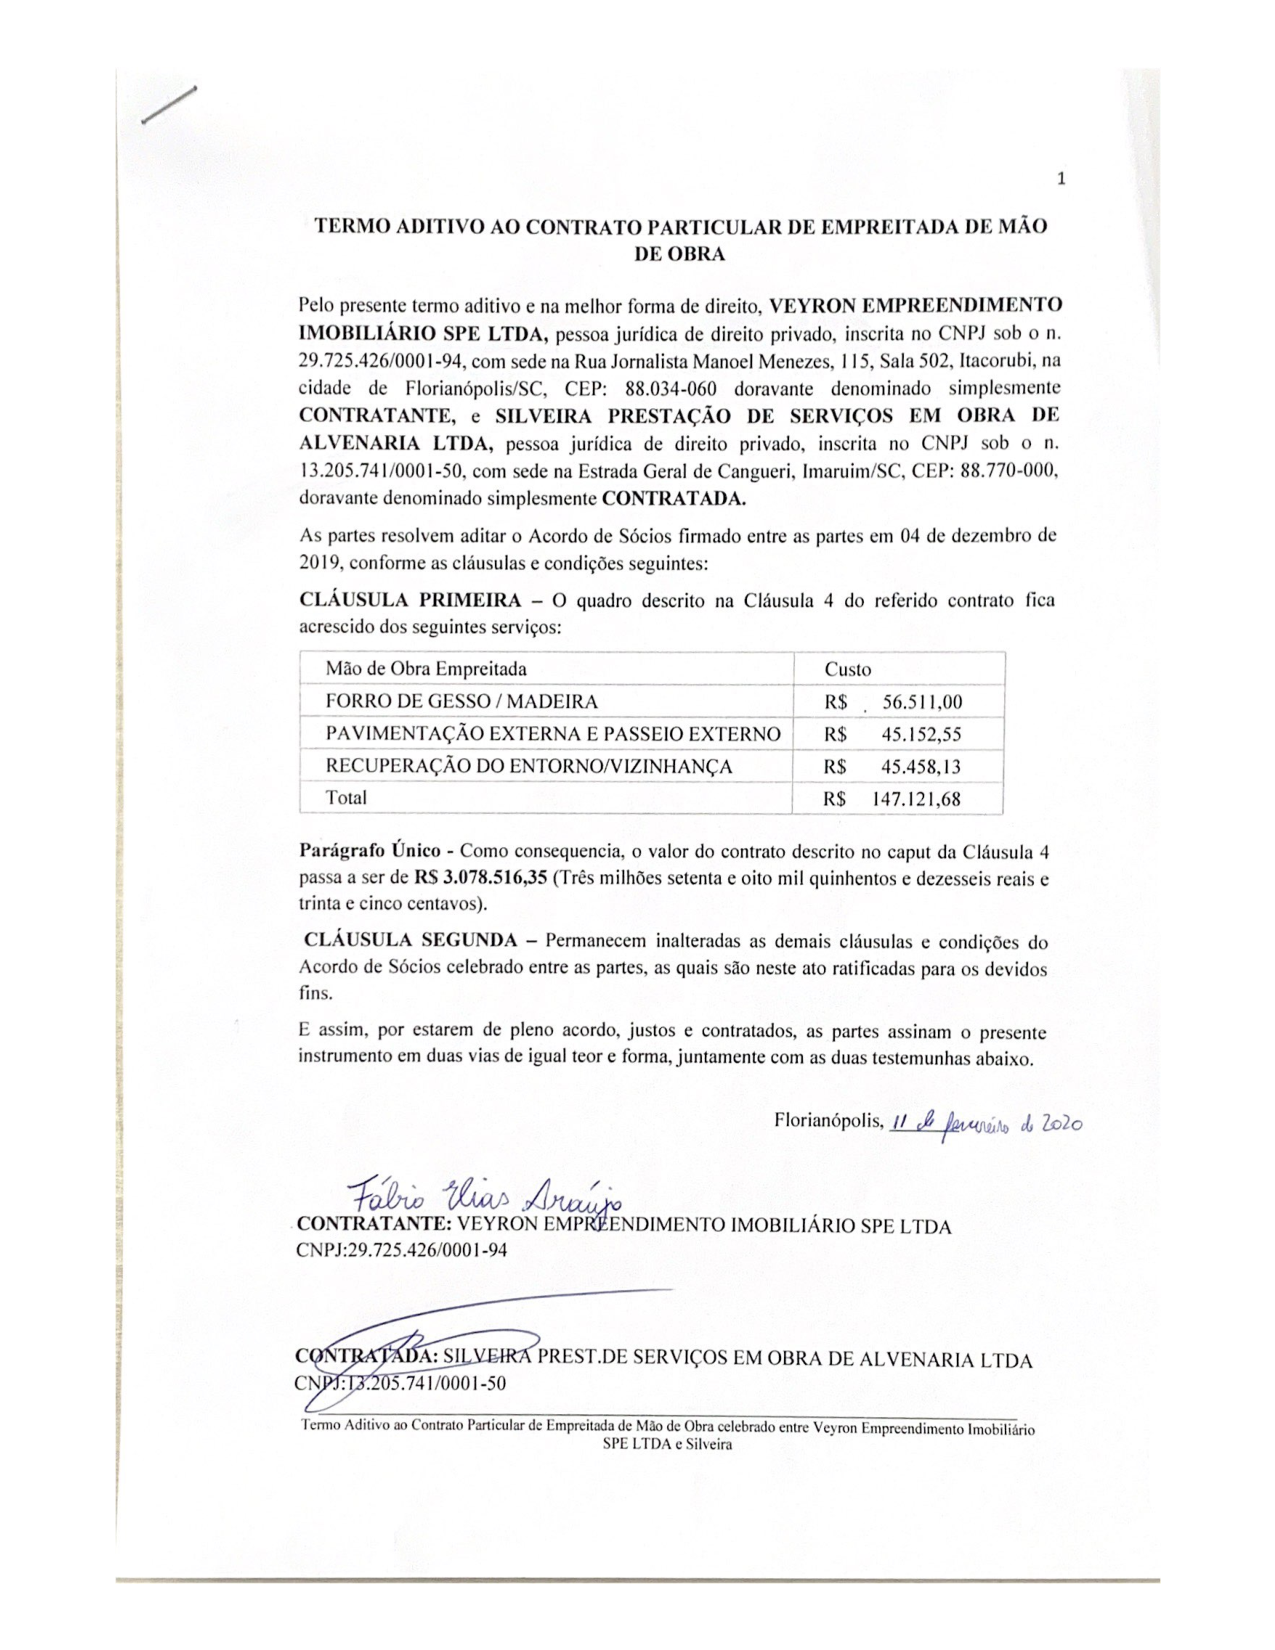
\includepdf[pages=-]{./refs/CT_DJ_Empreitada Globa - Aditivo.pdf}

\bookmarksetup{startatroot}

\chapter*{ANEXO III}\label{anexo-iii}
\addcontentsline{toc}{chapter}{ANEXO III}

\markboth{ANEXO III}{ANEXO III}

\includepdf[pages=-]{./refs/Contrato Veyron DJ - Assinado.pdf}

\bookmarksetup{startatroot}

\chapter*{ANEXO IV}\label{anexo-iv}
\addcontentsline{toc}{chapter}{ANEXO IV}

\markboth{ANEXO IV}{ANEXO IV}

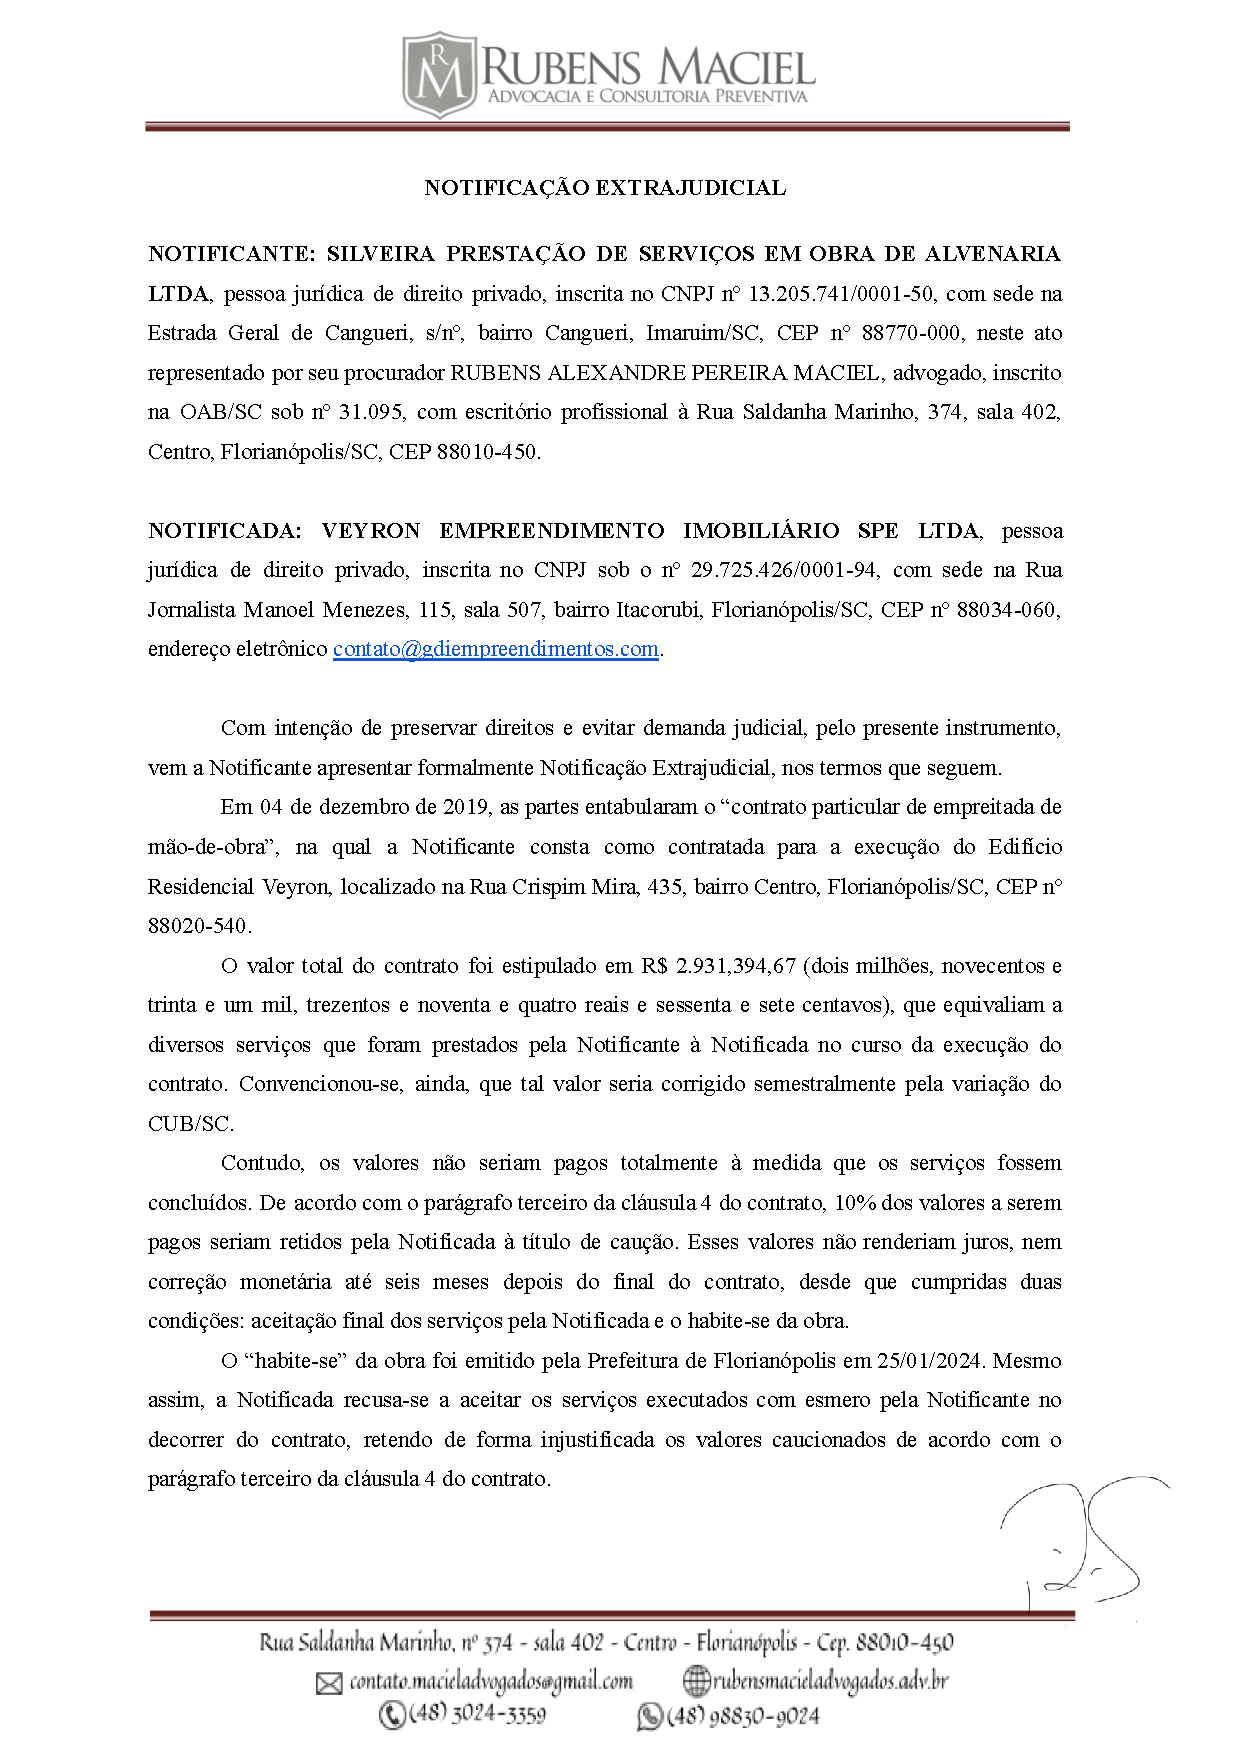
\includepdf[pages=-]{./refs/01_Notificação Extrajudicial_250822_152450.pdf}

\bookmarksetup{startatroot}

\chapter*{ANEXO V}\label{anexo-v}
\addcontentsline{toc}{chapter}{ANEXO V}

\markboth{ANEXO V}{ANEXO V}

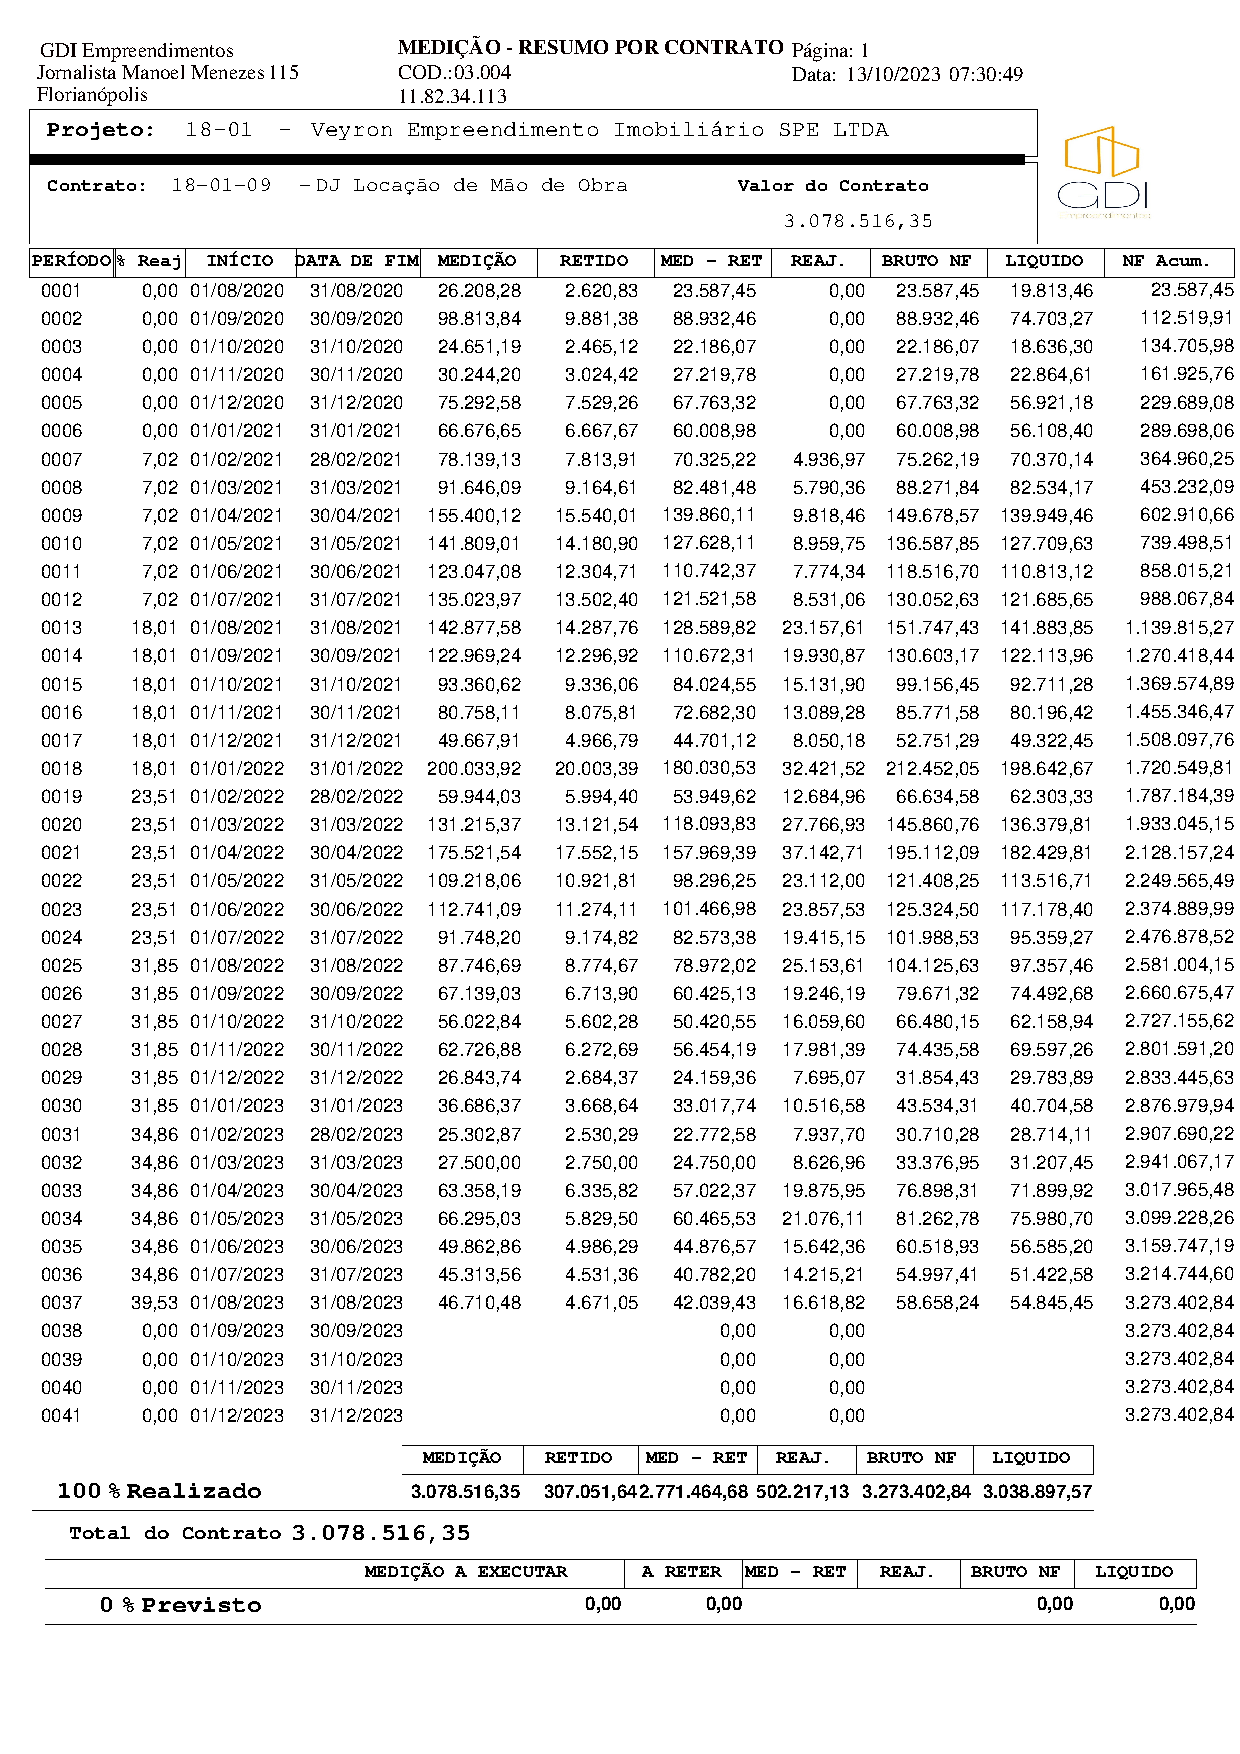
\includepdf[pages=-]{./refs/Resumo_Medicoes.pdf}

\bookmarksetup{startatroot}

\chapter*{ANEXO VI}\label{anexo-vi}
\addcontentsline{toc}{chapter}{ANEXO VI}

\markboth{ANEXO VI}{ANEXO VI}

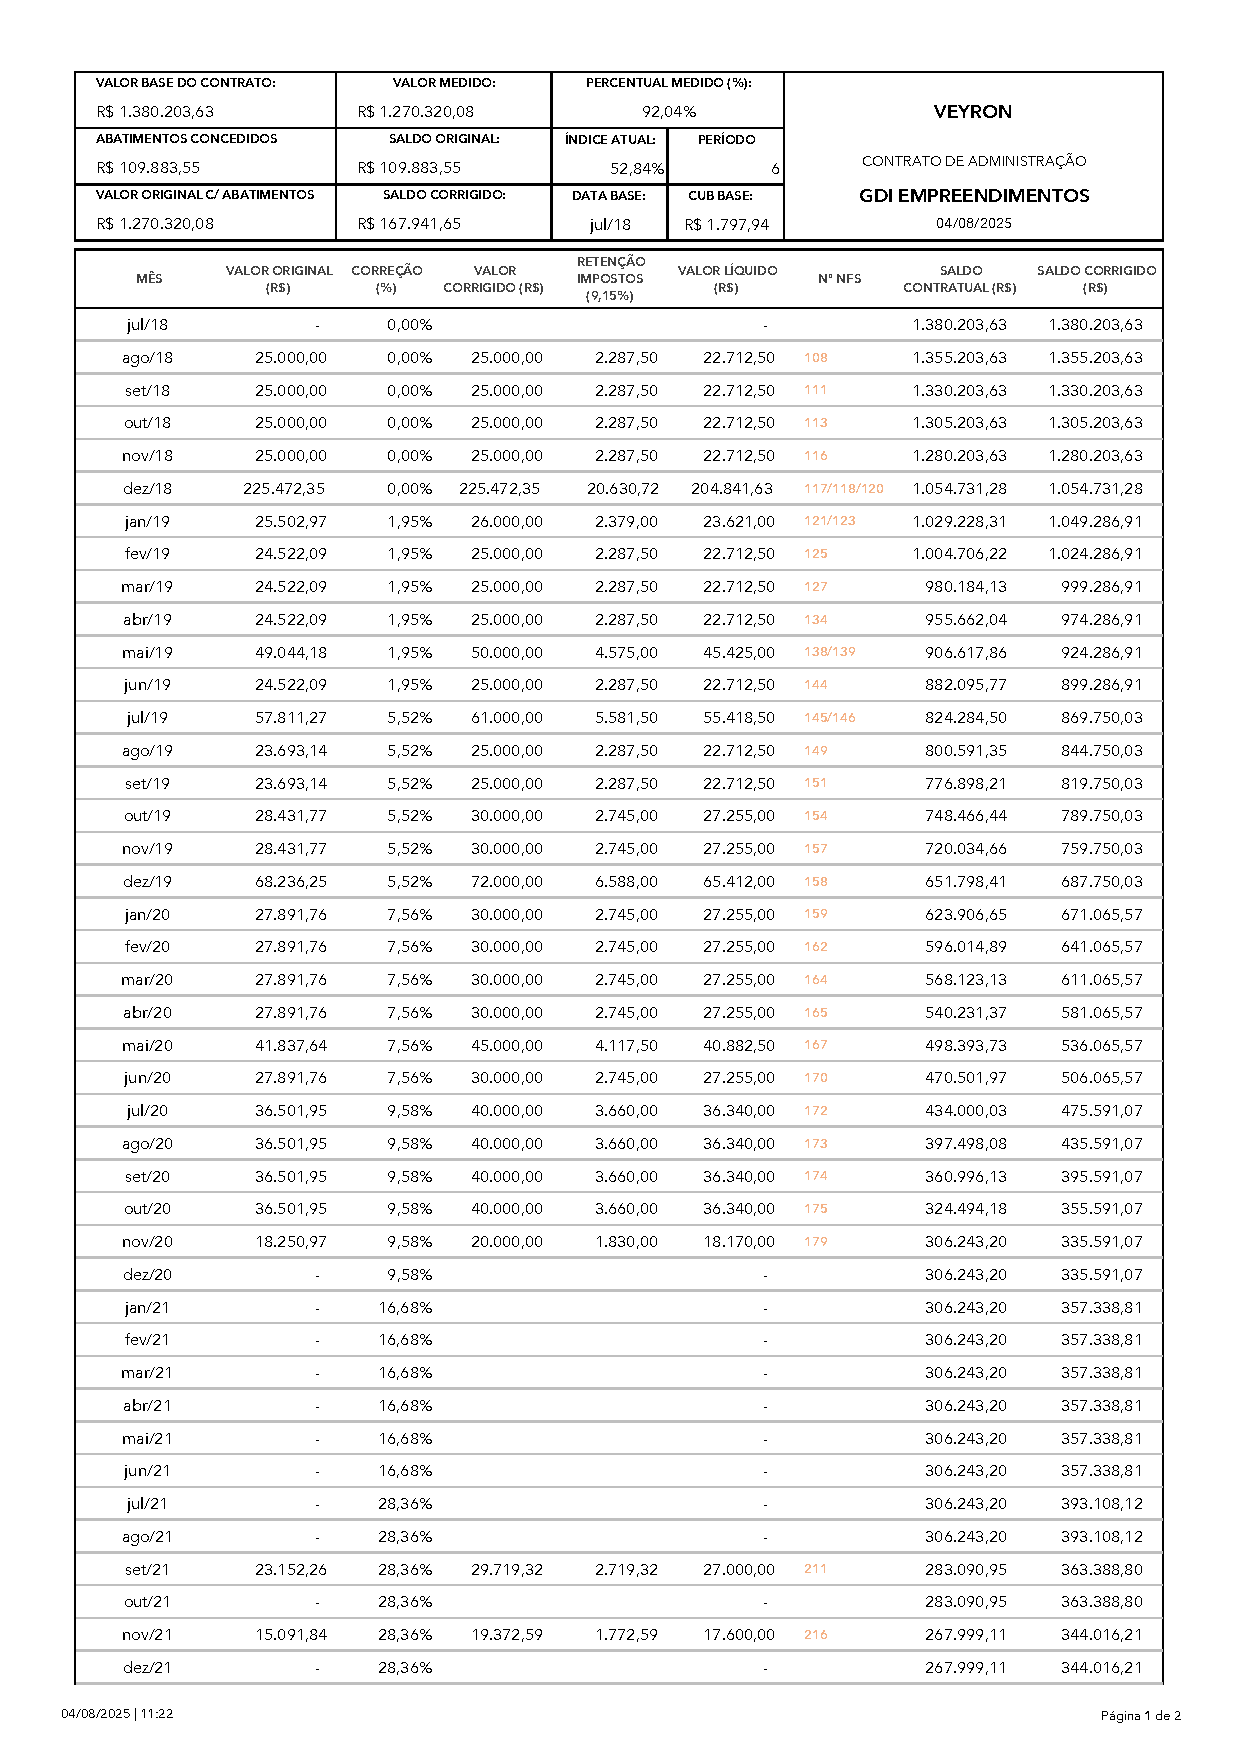
\includepdf[pages=-]{./refs/NF GDI/Resumo_GDI.pdf}




\end{document}
